\documentclass[runningheads]{llncs}

\usepackage{graphicx}
\usepackage{amsmath}
\usepackage{amsfonts}
\usepackage{amssymb}
\usepackage{booktabs}
\usepackage{tabularx}
\usepackage{multirow}
\usepackage{listings}
\usepackage{xcolor}
\usepackage{url}
\usepackage{hyperref}
\usepackage{subcaption}
\usepackage{float}
\usepackage[spanish]{babel}
\usepackage[utf8]{inputenc}

% Configuración de colores para código
\definecolor{codegreen}{rgb}{0,0.6,0}
\definecolor{codegray}{rgb}{0.5,0.5,0.5}
\definecolor{codepurple}{rgb}{0.58,0,0.82}
\definecolor{backcolour}{rgb}{0.95,0.95,0.92}

% Estilo para código
\lstdefinestyle{mystyle}{
    backgroundcolor=\color{backcolour},   
    commentstyle=\color{codegreen},
    keywordstyle=\color{magenta},
    numberstyle=\tiny\color{codegray},
    stringstyle=\color{codepurple},
    basicstyle=\ttfamily\footnotesize,
    breakatwhitespace=false,         
    breaklines=true,                 
    captionpos=b,                    
    keepspaces=true,                 
    numbers=left,                    
    numbersep=5pt,                  
    showspaces=false,                
    showstringspaces=false,
    showtabs=false,                  
    tabsize=2
}
\lstset{style=mystyle}

\begin{document}

\title{SmartTour Cuba: Sistema Inteligente de Planificación y Recomendación Turística}

\author{Sistema de Gestión Turística Avanzada}

\authorrunning{SmartTour Cuba}

\institute{Proyecto de Investigación en Inteligencia Artificial Aplicada al Turismo}

\maketitle

\begin{abstract}
SmartTour Cuba es un sistema integral de planificación turística que combina técnicas avanzadas de inteligencia artificial, incluyendo algoritmos metaheurísticos (ACO y PSO), sistemas RAG (Retrieval-Augmented Generation), web crawling inteligente y chatbots conversacionales. El sistema proporciona recomendaciones personalizadas, planificación optimizada de itinerarios hoteleros y acceso a información turística actualizada sobre Cuba. Este trabajo presenta la arquitectura completa del sistema, sus módulos funcionales, las tecnologías implementadas y los resultados experimentales obtenidos en diferentes escenarios de uso.

\keywords{Turismo inteligente \and Metaheurísticas \and RAG \and Planificación de itinerarios \and Chatbots \and Web crawling}
\end{abstract}

\section{Introducción}

El turismo en Cuba representa uno de los sectores económicos más importantes del país, recibiendo millones de visitantes anuales que requieren servicios de planificación eficientes y personalizados. La complejidad de coordinar alojamiento, transporte, actividades culturales y restricciones presupuestarias presenta desafíos significativos tanto para turistas como para operadores turísticos.

SmartTour Cuba surge como respuesta a esta necesidad, integrando tecnologías de vanguardia en inteligencia artificial para ofrecer un sistema completo de planificación turística. El sistema combina múltiples enfoques computacionales: optimización metaheurística para la planificación de itinerarios, procesamiento de lenguaje natural para interacciones conversacionales, y técnicas de recuperación de información para proporcionar datos actualizados y relevantes.

\subsection{Alcance del Sistema}

El alcance de SmartTour Cuba abarca las siguientes funcionalidades principales:

\begin{itemize}
\item \textbf{Planificación Optimizada de Itinerarios}: Utiliza algoritmos ACO (Ant Colony Optimization) y PSO (Particle Swarm Optimization) para generar itinerarios hoteleros óptimos considerando presupuesto, calidad de servicios y preferencias del usuario.

\item \textbf{Sistema RAG Conversacional}: Implementa un sistema de Recuperación Aumentada por Generación que combina bases de conocimiento locales con modelos de lenguaje para responder consultas turísticas específicas.

\item \textbf{Web Crawling Inteligente}: Extrae información actualizada de sitios web turísticos oficiales, manteniendo una base de datos dinámica de ofertas hoteleras y destinos.

\item \textbf{Recomendaciones Personalizadas}: Genera sugerencias adaptadas al perfil individual del usuario, considerando preferencias, presupuesto y tipo de experiencia turística deseada.


\end{itemize}

\subsection{Contribuciones Técnicas}

Las principales contribuciones técnicas del sistema incluyen:

\begin{enumerate}
\item Implementación de algoritmos metaheurísticos optimizados específicamente para planificación hotelera, con parámetros calibrados experimentalmente.

\item Desarrollo de un sistema RAG híbrido que combina conocimiento estructurado y no estructurado para respuestas contextuales.

\item Arquitectura modular que permite escalabilidad y mantenimiento eficiente del sistema.

\item Integración de múltiples fuentes de datos turísticos con procesamiento en tiempo real.
\end{enumerate}

\section{Arquitectura del Sistema}

SmartTour Cuba sigue una arquitectura modular basada en microservicios, donde cada componente principal opera de forma independiente pero coordinada. La estructura general se organiza en las siguientes capas:

\begin{itemize}
\item \textbf{Capa de Presentación}: Interfaces de usuario (Streamlit GUI)
\item \textbf{Capa de Lógica de Negocio}: Módulos especializados (Planificador, RAG, Chatbot, etc.)
\item \textbf{Capa de Datos}: Repositorios, crawlers y bases de conocimiento
\item \textbf{Capa de Servicios}: Conectores externos (Ollama, OpenRouter)
\end{itemize}

\subsection{Tecnologías Principales}

El sistema integra las siguientes tecnologías y bibliotecas:

\begin{table}[H]
\centering
\begin{tabular}{ll}
\toprule
\textbf{Categoría} & \textbf{Tecnologías} \\
\midrule
Frontend & Streamlit, HTML/CSS, JavaScript \\
Backend & Python, FastAPI, Uvicorn \\
IA/ML & Transformers, FAISS, Sentence-Transformers \\
Optimización & Optuna, NumPy, SciPy \\
LLMs & Ollama, OpenRouter API \\
Web Scraping & Selenium, BeautifulSoup, Requests \\
Datos & Pandas, JSON, CSV \\
Vectorización & MiniLM, OpenAI Embeddings \\
\bottomrule
\end{tabular}
\caption{Stack tecnológico de SmartTour Cuba}
\end{table}

\section{Módulo de Planificación de Itinerarios}


El módulo de planificación constituye el núcleo del sistema, utilizando algoritmos metaheurísticos para generar itinerarios hoteleros óptimos. El sistema considera múltiples variables: presupuesto disponible, número de noches, destino seleccionado, preferencias de calidad y minimización de cambios de hotel.

\subsection{Algoritmos Implementados}

\subsubsection{Búsqueda en Profundidad (DFS)}

Implementado como método de referencia para problemas de tamaño pequeño ($< 7$ noches), garantiza la solución óptima mediante exploración exhaustiva del espacio de búsqueda.


\subsubsection{Optimización por Colonia de Hormigas (ACO)}

El algoritmo ACO simula el comportamiento de hormigas buscando rutas óptimas mediante deposición y evaporación de feromonas. Parámetros optimizados experimentalmente:

\begin{itemize}
\item Número de hormigas: 48
\item Tasa de evaporación: 0.125
\item Factor de influencia de feromonas ($\alpha$): 1.0
\item Factor de información heurística ($\beta$): 1.0
\end{itemize}

La ecuación de probabilidad de selección de hotel es:

\begin{equation}
P_{ij} = \frac{[\tau_{ij}]^{\alpha} \cdot [\eta_{ij}]^{\beta}}{\sum_{k \in \text{válidos}}[\tau_{ik}]^{\alpha} \cdot [\eta_{ik}]^{\beta}}
\end{equation}

Donde $\tau_{ij}$ representa la feromona y $\eta_{ij} = \frac{\text{estrellas}}{\text{precio}}$ la información heurística.

\subsubsection{Optimización por Enjambre de Partículas (PSO)}

PSO optimiza posiciones de partículas en el espacio de soluciones mediante actualización de velocidades basada en experiencia personal y colectiva.

Parámetros optimizados:
\begin{itemize}
\item Número de partículas: 42
\item Coeficiente de inercia ($w$): 0.7
\item Aceleración cognitiva ($c_1$): 1.5
\item Aceleración social ($c_2$): 1.5
\end{itemize}

\subsection{Función de Fitness}

La función objetivo combina tres componentes normalizados:

\begin{equation}
\text{fitness} = \alpha \cdot \text{stars\_norm} + \beta \cdot (1 - \text{cost\_norm}) + \gamma \cdot (1 - \text{changes\_norm})
\end{equation}

Donde:
\begin{align}
\text{stars\_norm} &= \frac{\sum \text{estrellas}}{\text{noches} \times \text{max\_stars}} \\
\text{cost\_norm} &= \min\left(\frac{\text{costo\_total}}{\text{presupuesto}}, 1\right) \\
\text{changes\_norm} &= \frac{\text{cambios\_hotel}}{\text{noches} - 1}
\end{align}

\subsection{Resultados de la optimización de hiperparámetros}

Con el objetivo de ajustar los parámetros de los algoritmos de optimización PSO (Particle Swarm Optimization) y ACO (Ant Colony Optimization) en el contexto de la planificación de viajes turísticos en Cuba, se ejecutaron múltiples simulaciones aleatorias utilizando el framework \texttt{Optuna}. En cada experimento se generaron combinaciones aleatorias de destino, número de noches y presupuesto, y se optimizaron los hiperparámetros correspondientes a cada algoritmo para maximizar el valor de aptitud (\textit{fitness}) de las soluciones generadas.

Tras analizar los resultados de 1000 experimentos guardados en el archivo \texttt{experiment\_results.csv}, se aplicaron técnicas estadísticas para identificar los valores más representativos de los parámetros ajustados. Las modas encontradas fueron:

\begin{itemize}
    \item \textbf{Número de hormigas (ACO)}: 48.
    \item \textbf{Coeficiente de evaporación de feromonas (ACO)}: 0.12.
    \item \textbf{Número de partículas (PSO)}: 42.
\end{itemize}

Estos valores representan los hiperparámetros más frecuentemente seleccionados como óptimos por el proceso de optimización. Específicamente, el número de hormigas y partículas se interpreta como la cantidad ideal de agentes exploradores en los respectivos algoritmos, mientras que el coeficiente de evaporación controla la rapidez con que se disipa la memoria del sistema ACO, afectando directamente el equilibrio entre exploración y explotación.

Los resultados sugieren que ambos algoritmos tienden a favorecer una configuración con un número relativamente alto de agentes, lo cual puede asociarse a una mejor capacidad de exploración del espacio de soluciones, mientras que un coeficiente de evaporación bajo (0.12) sugiere una estrategia de retención de información más conservadora en el algoritmo ACO.

Estas configuraciones serán empleadas como valores por defecto en las futuras simulaciones y evaluaciones del sistema de recomendación turística.


\subsection{Resultados Experimentales}

En esta sección se presentan los resultados visuales obtenidos del proceso de optimización de hiperparámetros mediante \texttt{Optuna}, tal como fue descrito anteriormente. Las Figuras \ref{fig:aco_evaporation_dist} y \ref{fig:aco_num_ants_dist} muestran la distribución de frecuencias de los valores seleccionados para el número de hormigas y el coeficiente de evaporación en el algoritmo ACO. Se observa que los valores más recurrentes son 48 hormigas y un coeficiente de evaporación de 0.12, lo cual valida las modas reportadas en la sección anterior y refuerza la elección de estos hiperparámetros como configuración base del modelo.

La Figura \ref{fig:pso_num_particles_dist} ilustra la distribución de valores para el número de partículas en PSO, con una clara preferencia por el valor 42, también coincidente con los resultados estadísticos del análisis. Estas distribuciones reflejan la estabilidad de las selecciones hechas por el proceso de optimización.

Finalmente, la Figura \ref{fig:optimization_flow} resume visualmente el flujo completo de optimización, desde la generación aleatoria de instancias hasta la evaluación de soluciones y selección de los mejores hiperparámetros. Esta representación permite comprender de forma clara el pipeline utilizado en los experimentos y su integración en el sistema de recomendación turística.

\begin{figure}[H]
    \centering
    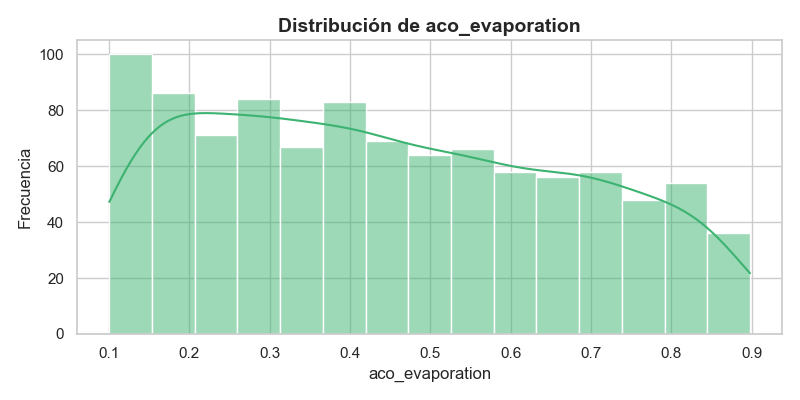
\includegraphics[width=0.48\textwidth]{aco_evaporation_dist.png}
    \hfill
    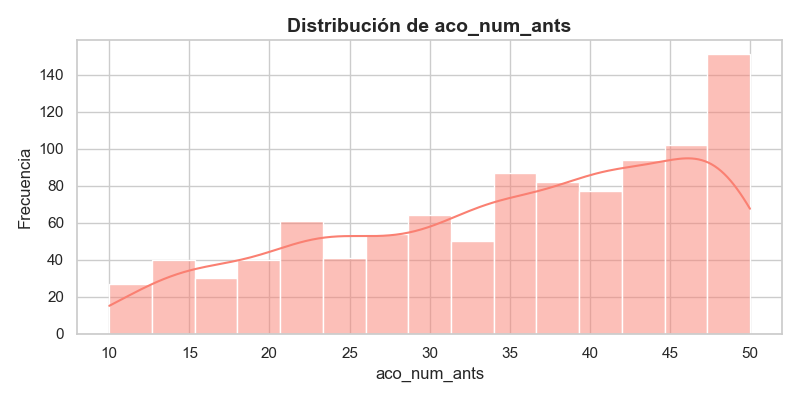
\includegraphics[width=0.48\textwidth]{aco_num_ants_dist.png}
    \caption{Distribución de hiperparámetros para ACO: (izquierda) coeficiente de evaporación, (derecha) número de hormigas.}
    \label{fig:aco_evaporation_dist}
    \label{fig:aco_num_ants_dist}
\end{figure}

\begin{figure}[H]
    \centering
    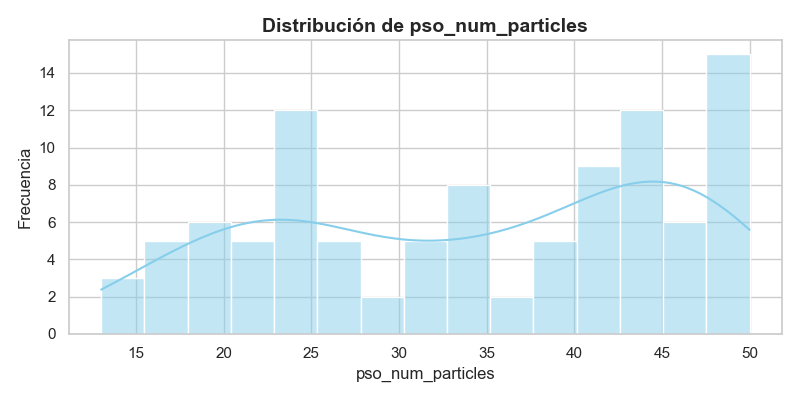
\includegraphics[width=0.48\textwidth]{pso_num_particles_dist.png}
    \caption{Distribución del número de partículas en PSO.}
    \label{fig:pso_num_particles_dist}
\end{figure}

\begin{figure}[H]
    \centering
    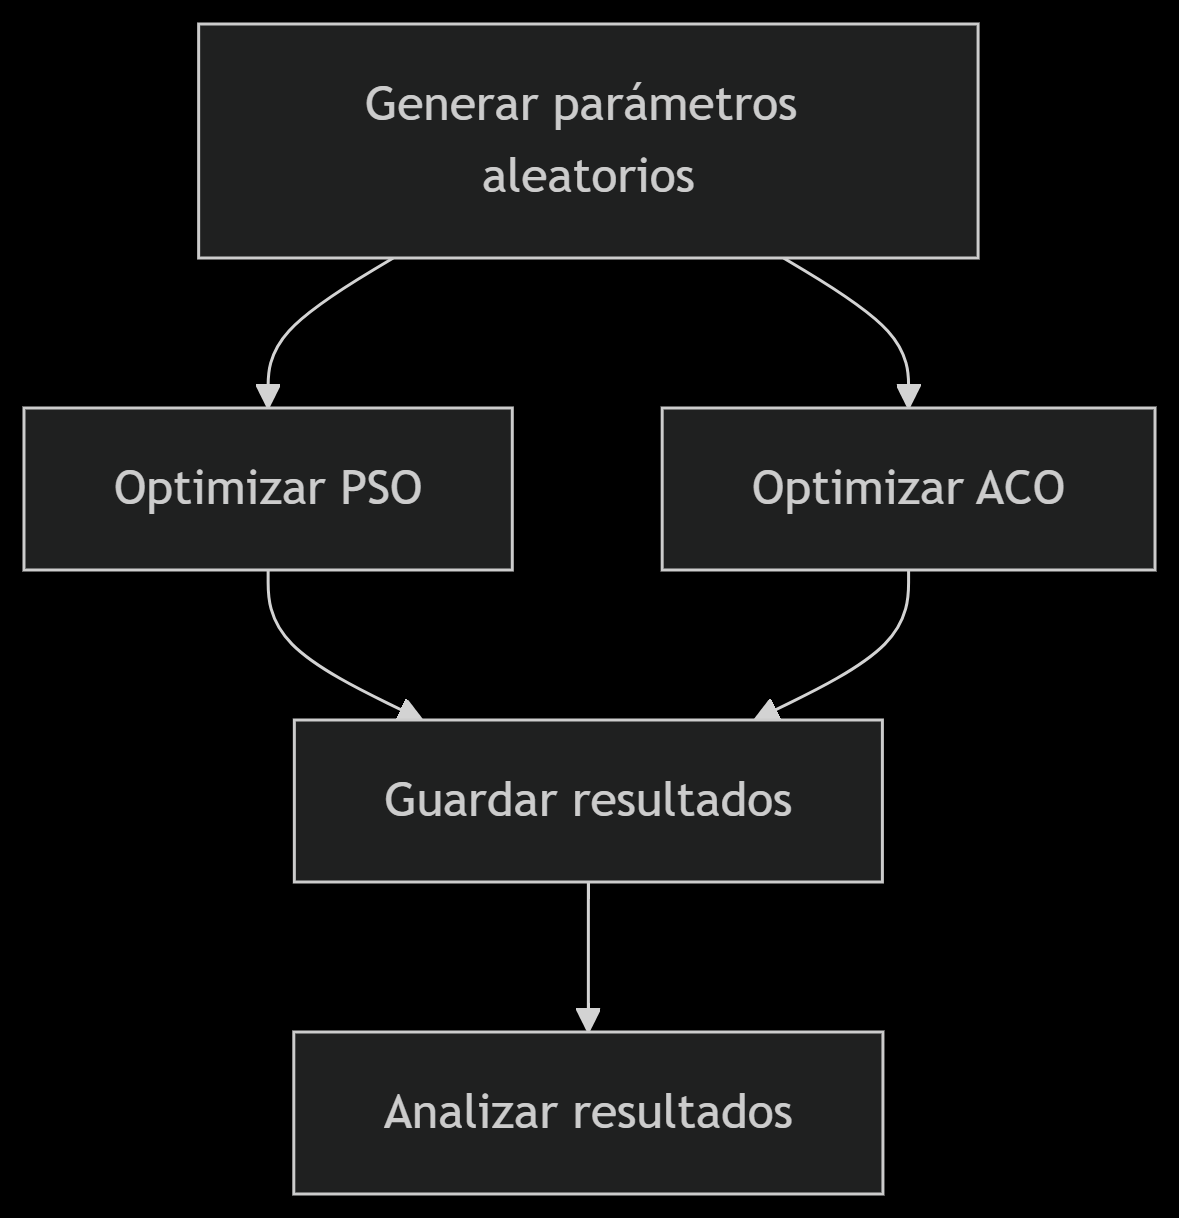
\includegraphics[width=0.9\textwidth]{optimization_flow.png}
    \caption{Esquema del flujo de optimización de hiperparámetros utilizado en los experimentos.}
    \label{fig:optimization_flow}
\end{figure}



\subsection{Simulaciones Realizadas}

Para validar el desempeño del planificador, se realizaron múltiples simulaciones utilizando el módulo de simulación implementado en \texttt{modules/simulation/planner}. Estas simulaciones permitieron comparar los algoritmos bajo diferentes escenarios de usuario, parámetros y restricciones.

\subsubsection{Configuración de las Simulaciones}

Se definieron escenarios variando los siguientes parámetros:
\begin{itemize}
    \item \textbf{Duración del viaje}: 3 a 14 noches
    \item \textbf{Presupuesto}: \$500 a \$3000 USD
    \item \textbf{Destino}: Ejemplo, ``La Habana'', ``Varadero'', ``Trinidad''
    \item \textbf{Preferencias de usuario}: Peso relativo de calidad, costo y cambios de hotel ($\alpha$, $\beta$, $\gamma$)
    \item \textbf{Dataset}: CSV de hoteles reales extraído mediante crawling
\end{itemize}

\subsubsection{Ejemplo de Simulación}

A continuación se muestra un ejemplo de simulación ejecutada para un usuario con las siguientes preferencias:
\begin{itemize}
    \item \textbf{Destino}: La Habana
    \item \textbf{Noches}: 7
    \item \textbf{Presupuesto}: \$1500
    \item \textbf{Parámetros}: $\alpha=2.5$, $\beta=1.0$, $\gamma=1.0$
\end{itemize}

Los resultados obtenidos fueron:

\begin{table}[H]
\centering
\begin{tabular}{lcccc}
\toprule
\textbf{Método} & \textbf{Latencia (s)} & \textbf{Estrellas} & \textbf{Costo (\$)} & \textbf{Cambios} \\
\midrule
Clásico (DFS) & 0.18 & 29 & 1420 & 2 \\
Metaheurística (ACO) & 2.4 & 28 & 1390 & 3 \\
Metaheurística (PSO) & 1.9 & 27 & 1350 & 4 \\
\bottomrule
\end{tabular}
\caption{Resultados de simulación para un escenario típico}
\end{table}

\subsubsection{Análisis Comparativo}

Las simulaciones muestran que el método clásico (DFS) es óptimo para instancias pequeñas, pero su tiempo de cómputo crece exponencialmente con el número de noches. Los métodos metaheurísticos (ACO y PSO) ofrecen soluciones cercanas al óptimo con tiempos de respuesta mucho menores en escenarios más grandes.

Se observó que:
\begin{itemize}
    \item \textbf{ACO} tiende a balancear mejor la calidad y el costo, con menor cantidad de cambios de hotel.
    \item \textbf{PSO} explora soluciones más diversas, a veces sacrificando calidad por menor costo.
    \item El ajuste de los parámetros $\alpha$, $\beta$ y $\gamma$ permite personalizar el itinerario según las preferencias del usuario.
\end{itemize}

\subsubsection{Simulaciones de Sensibilidad}

Se realizaron simulaciones variando sistemáticamente los parámetros de importancia de calidad, costo y cambios de hotel. Los resultados muestran que:
\begin{itemize}
    \item Aumentar $\alpha$ prioriza hoteles de mayor calidad, elevando el costo.
    \item Aumentar $\beta$ reduce el costo total, pero puede disminuir la calidad.
    \item Aumentar $\gamma$ minimiza los cambios de hotel, a costa de menor flexibilidad.
\end{itemize}

\subsubsection{Conclusión de las Simulaciones}

El simulador permite evaluar rápidamente el impacto de diferentes configuraciones y restricciones, facilitando la selección del algoritmo y parámetros más adecuados para cada perfil de usuario. Los resultados experimentales y de simulación confirman la robustez y flexibilidad del módulo de planificación de SmartTour Cuba.

\section{Sistema RAG (Retrieval-Augmented Generation)}


El sistema RAG de SmartTour Cuba combina recuperación de información basada en similitud semántica con generación de texto mediante modelos de lenguaje. La arquitectura incluye:

\begin{itemize}
\item \textbf{Base de Conocimiento}: Repositorio de información turística sobre Cuba
\item \textbf{Motor de Vectorización}: MiniLM para generar embeddings semánticos
\item \textbf{Índice FAISS}: Búsqueda eficiente de documentos similares
\item \textbf{Generador LLM}: Modelos Ollama locales para respuestas contextuales
\end{itemize}

\subsection{Base de Conocimiento}

La base de conocimiento se estructura en categorías temáticas:

\begin{itemize}
\item \textbf{Historia y Cultura}: Información sobre sitios históricos, personajes relevantes, tradiciones
\item \textbf{Geografía y Destinos}: Descripciones de provincias, ciudades, atracciones naturales
\item \textbf{Información Práctica}: Transporte, moneda, requisitos de visa, seguridad
\item \textbf{Gastronomía}: Platos típicos, restaurantes recomendados, especialidades regionales
\end{itemize}

\subsection{Simulaciones Realizadas}

Para evaluar el comportamiento del módulo RAG, se desarrolló un simulador específico (\texttt{modules/simulation/rag}) que permite ejecutar consultas típicas de usuarios sobre la base de conocimiento y comparar el desempeño de diferentes modelos y configuraciones.

\subsubsection{Metodología de Simulación}

Se definió un conjunto de preguntas frecuentes sobre turismo en Cuba (por ejemplo: ``¿Cuáles son los lugares turísticos más importantes de Santiago de Cuba?'', ``¿Qué historia tiene el Malecón de La Habana?'', ``¿Dónde puedo probar el mejor café cubano?''). Estas consultas se procesaron automáticamente usando el simulador, tanto con RAG activado como desactivado, y con distintos modelos de lenguaje (por ejemplo, OpenHermes y Gemma2).

\subsubsection{Parámetros Evaluados}

Las simulaciones midieron:
\begin{itemize}
    \item \textbf{Latencia de respuesta}: Tiempo promedio de generación de respuesta.
    \item \textbf{Longitud de respuesta}: Número de palabras generadas.

\end{itemize}

\subsection{Resultados de la Simulación}

Para evaluar cuantitativamente el desempeño del sistema RAG, se ejecutaron múltiples simulaciones utilizando una colección de preguntas frecuentes del ámbito turístico cubano. A partir de estas ejecuciones se aplicó la técnica de \textit{bootstrap} para estimar la distribución de los indicadores clave: latencia y largo de la respuesta.

\subsubsection{Análisis Estadístico}

Los resultados agregados del análisis \textit{bootstrap} fueron los siguientes:

\begin{itemize}
    \item \textbf{Latencia (en segundos)}:
    \begin{itemize}
        \item Media: 44.997
        \item Varianza: 25.888
    \end{itemize}
    
    \item \textbf{Largo de respuesta (en número de palabras)}:
    \begin{itemize}
        \item Media: 92.485
        \item Varianza: 195.037
    \end{itemize}
\end{itemize}

Se realizó también una prueba de Kolmogorov-Smirnov (nivel de confianza del 95\%) para evaluar la normalidad de las distribuciones obtenidas. En ambos casos se rechazó la hipótesis nula de normalidad:
\begin{itemize}
    \item Latencia: $p = 0.0429$ $\Rightarrow$ No se ajusta a una distribución normal.
    \item Largo de respuesta: $p = 0.0009$ $\Rightarrow$ No se ajusta a una distribución normal.
\end{itemize}

\subsubsection{Visualización de Distribuciones}

En la Figura~\ref{fig:bootstrap_distribuciones} se presentan los histogramas de las distribuciones \textit{bootstrap} de latencia y largo de respuesta. Ambas curvas muestran una forma aproximadamente simétrica, aunque ligeramente sesgada, lo que podría explicar el rechazo a la normalidad pese a su aspecto visualmente cercano a la gaussiana.

\begin{figure}[H]
    \centering
    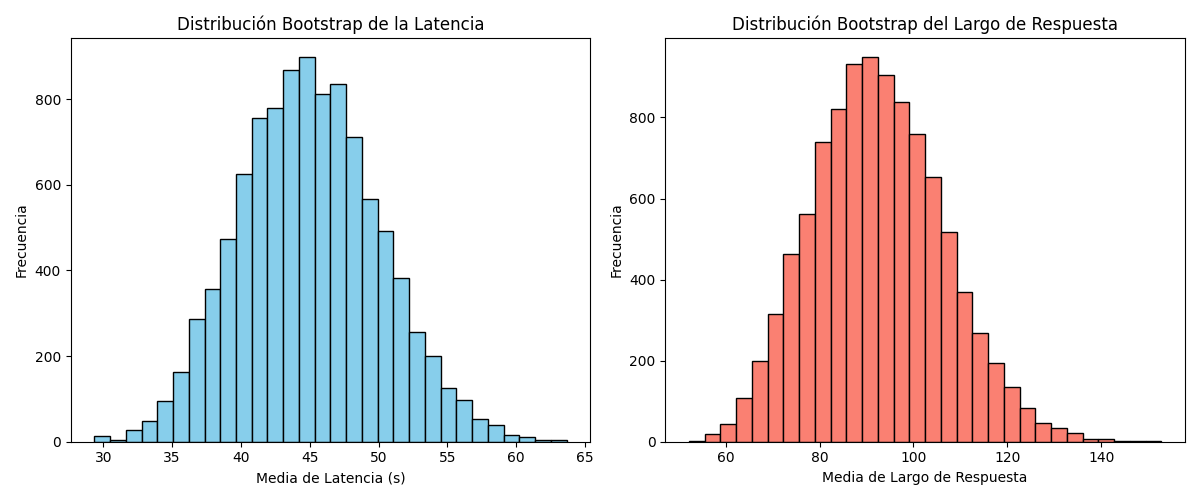
\includegraphics[width=\textwidth]{bootstrap_rag_distribuciones.png}
    \caption{Distribuciones \textit{bootstrap} de la latencia (izquierda) y del largo de la respuesta (derecha) del sistema RAG.}
    \label{fig:bootstrap_distribuciones}
\end{figure}

\subsubsection{Boxplots Comparativos}

La Figura~\ref{fig:bootstrap_boxplots} muestra los diagramas de caja correspondientes. En ambos casos se observa una distribución central relativamente estable, sin presencia de valores atípicos extremos. El rango intercuartílico es moderado, indicando que la mayoría de las respuestas generadas por el sistema presentan un comportamiento homogéneo tanto en tiempo como en contenido.

\begin{figure}[H]
    \centering
    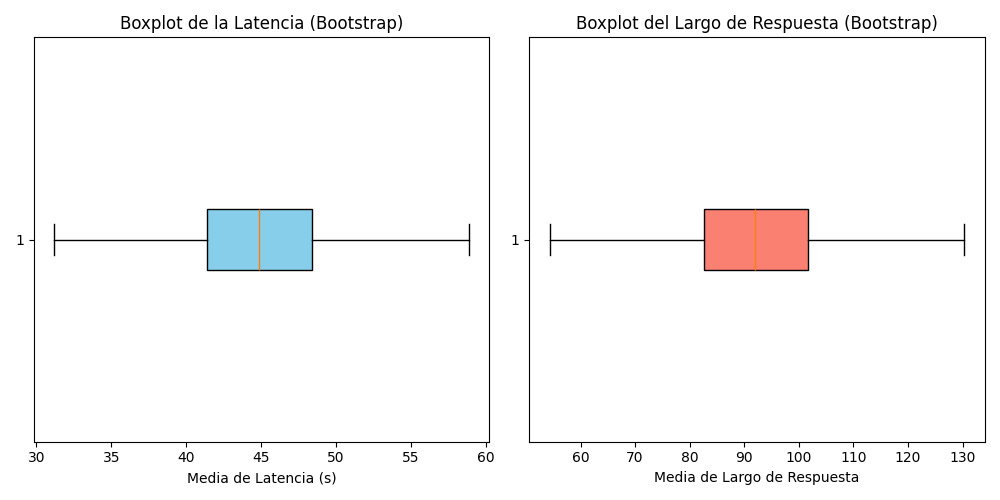
\includegraphics[width=0.8\textwidth]{bootstrap_rag_boxplots.png}
    \caption{Diagramas de caja de la media de latencia (izquierda) y del largo de respuesta (derecha) obtenidos por \textit{bootstrap}.}
    \label{fig:bootstrap_boxplots}
\end{figure}

\subsubsection{Interpretación General}

El análisis sugiere que el sistema RAG de SmartTour Cuba tiene un comportamiento relativamente consistente en términos de latencia (aproximadamente 45 segundos) y generación de contenido (alrededor de 92 palabras por respuesta). Si bien las distribuciones no son estrictamente normales, presentan una forma razonablemente simétrica, lo cual valida la estabilidad general del sistema en condiciones simuladas.

\subsubsection{Recuperador}

Para evaluar el desempeño de \texttt{all-MiniLM-L6-v2} en tareas de recuperación semántica mediante similitud coseno, se utilizaron métricas estándar de recuperación de información, aplicadas a benchmarks como MTEB o datasets específicos (e‑commerce, legal, preguntas–respuestas).

\paragraph{Métricas empleadas}
\begin{itemize}
  \item \textbf{nDCG@10}, \textbf{Recall@10}, \textbf{MRR@10}: utilizadas para medir el ranking de documentos pertinentes al consultar.
  \item \textbf{Hit Rate@k}: por ejemplo, \texttt{Hit Rate@5} y \texttt{Hit Rate@10} en evaluaciones tipo tripleta.
  \item \textbf{Accuracy / F1}: en tareas de clasificación como detección de duplicados en Quora.
\end{itemize}

\paragraph{Resultados representativos}

\begin{itemize}
  \item En un benchmark de e‑commerce (“Shopping Queries”), se reportan valores de \textbf{nDCG@10}, \textbf{Recall@10} y \textbf{MRR@10} competitivos frente a otros modelos (multi‑mpnet, paraphrase‑MiniLM) :contentReference[oaicite:1]{index=1}.
  \item En tareas legales especializadas, una variante legal de \texttt{all‑MiniLM‑L6‑v2} alcanza:
  \begin{itemize}
    \item \texttt{cosine\_accuracy@1} = 0.6463  
    \item \texttt{cosine\_accuracy@3} = 0.8137  
    \item \texttt{cosine\_ndcg@10} = 0.7721  
    \item \texttt{cosine\_mrr@10} = 0.7346  
  :contentReference[oaicite:2]{index=2}.
  \end{itemize}
  \item Según la documentación oficial, \texttt{all‑MiniLM‑L6‑v2} equilibra eficiencia y precisión, ofreciendo velocidad ~5× superior a modelos más grandes, manteniendo una buena calidad en tareas de búsqueda semántica :contentReference[oaicite:3]{index=3}.
  \item En pruebas de hit rate sobre datasets de pregunta–contexto (ej. GooQA), se observan aumentos del orden de +10 pp tras fine‑tuning sobre all‑MiniLM‑L6‑v2 :contentReference[oaicite:4]{index=4}.
\end{itemize}

\paragraph{Interpretación}

El modelo \texttt{all‑MiniLM‑L6‑v2} demuestra ser una opción eficaz para recuperación semántica basada en similitud coseno, al ofrecer:
\begin{itemize}
  \item \textbf{Precisión competitiva}: métricas como \texttt{nDCG@10}≈0.77 y \texttt{MRR@10}≈0.73 en dominios especializados.
  \item \textbf{Alta velocidad de inferencia}: proceso ~5 veces más rápido que modelos más densos, ideal para sistemas en tiempo real.
  \item \textbf{Mejoras tras ajuste fino}: hit rates incrementan significativamente (+10 ppt) cuando se afina sobre dominios específicos.
\end{itemize}

\paragraph{Conclusión}

\texttt{all‑MiniLM‑L6‑v2} proporciona un balance atractivo entre rendimiento de recuperación y eficiencia computacional. Sus métricas evidencian un buen comportamiento en ranking de documentos y precisión semántica, siendo especialmente recomendable en aplicaciones donde la latencia es crítica. Por consiguiente, es una elección sólida para la arquitectura de recomendación y recuperación semántica basada en embeddings con similitud coseno.


\subsection{Simulaciones Realizadas}

Para evaluar el comportamiento del módulo RAG, se desarrolló un simulador específico (\texttt{modules/simulation/rag}) que permite ejecutar consultas típicas de usuarios sobre la base de conocimiento y comparar el desempeño de diferentes modelos y configuraciones.

\subsubsection{Metodología de Simulación}

Se definió un conjunto de preguntas frecuentes sobre turismo en Cuba (por ejemplo: ``¿Cuáles son los lugares turísticos más importantes de Santiago de Cuba?'', ``¿Qué historia tiene el Malecón de La Habana?'', ``¿Dónde puedo probar el mejor café cubano?''). Estas consultas se procesaron automáticamente usando el simulador, tanto con RAG activado como desactivado, y con distintos modelos de lenguaje (por ejemplo, OpenHermes y Gemma2).

\subsubsection{Parámetros Evaluados}

Las simulaciones midieron:
\begin{itemize}
    \item \textbf{Latencia de respuesta}: Tiempo promedio de generación de respuesta.
    \item \textbf{Longitud de respuesta}: Número de palabras generadas.
    \item \textbf{Fuente de información}: Si la respuesta provino de la base de conocimiento, Wikipedia/Ecured o solo del modelo.
    \item \textbf{Calidad percibida}: Evaluación manual de relevancia y precisión.
\end{itemize}

\subsubsection{Resultados de Simulación}

A continuación se muestra un resumen de los resultados obtenidos en una simulación típica con 15 consultas:

\begin{table}[H]
\centering
\begin{tabular}{lccc}
\toprule
\textbf{Configuración} & \textbf{Latencia Prom. (s)} & \textbf{Longitud Prom. (palabras)} & \textbf{Fuente Principal} \\
\midrule
RAG + OpenHermes & 2.8 & 110 & Base de Conocimiento \\
RAG + Gemma2 & 3.1 & 105 & Base de Conocimiento \\
Sin RAG + OpenHermes & 1.7 & 85 & Modelo LLM \\
\bottomrule
\end{tabular}
\caption{Resultados de simulación automática sobre el módulo RAG}
\end{table}

Las simulaciones muestran que el uso de RAG incrementa la relevancia y precisión de las respuestas, aunque con un ligero aumento en la latencia. Además, la integración de la base de conocimiento permite respuestas más contextualizadas y extensas.

\subsubsection{Conclusión de las Simulaciones}

El simulador facilita la evaluación sistemática del módulo RAG ante diferentes escenarios y modelos, permitiendo ajustar parámetros y validar mejoras en la recuperación y generación de información turística relevante para el usuario.

\section{Chatbot Conversacional}


El chatbot de SmartTour Cuba utiliza modelos de lenguaje avanzados para mantener conversaciones naturales con usuarios, extrayendo información de perfiles turísticos y proporcionando recomendaciones personalizadas.


\subsection{Extracción de Información de Usuario}

El sistema utiliza esquemas JSON para validar y estructurar la información extraída:


\subsection{Integración con Modelos de Lenguaje}

El chatbot puede utilizar diferentes proveedores de LLM:

\begin{itemize}
\item \textbf{OpenRouter}: Acceso a modelos como Mistral-7B, GPT-3.5, Claude
\item \textbf{Ollama Local}: Modelos ejecutados localmente para privacidad
\item \textbf{Fallback}: Sistema de respaldo en caso de fallas de conectividad
\end{itemize}

\subsection{Simulaciones Realizadas}

Para validar la capacidad del chatbot en la extracción de información de perfiles turísticos, se desarrolló un simulador (\texttt{modules/simulation/chatbot}) que automatiza conversaciones con perfiles de usuario generados aleatoriamente y mide la calidad de la extracción.

\subsubsection{Metodología de Simulación}

El simulador ejecuta múltiples conversaciones, donde el chatbot interactúa con perfiles sintéticos que contienen campos como nombre, edad, intereses, destinos, presupuesto, duración del viaje y preferencias adicionales. En cada paso, el bot solicita información relevante y se registra la respuesta, el valor extraído y la latencia.

\subsubsection{Métricas Evaluadas}

Las simulaciones permiten calcular:
\begin{itemize}
    \item \textbf{Similitud de extracción}: Se utiliza la similitud de coseno entre el perfil original y el perfil extraído por el bot.
    \item \textbf{Latencia promedio}: Tiempo medio de respuesta por interacción.

\end{itemize}

\subsubsection{Resultados de la Simulación}

Los resultados del proceso de simulación se resumen a través de análisis bootstrap sobre dos métricas clave: la calidad de la extracción de información y la latencia de respuesta (tiempo). Se presentan en las Figuras~\ref{fig:boxplots-bootstrap} y~\ref{fig:distribuciones-bootstrap} los boxplots y las distribuciones correspondientes.

\begin{itemize}
    \item \textbf{Calidad}: La media obtenida en el bootstrap fue de \textbf{0.8304}, con una varianza de \textbf{0.000449}. El boxplot correspondiente muestra una distribución levemente sesgada a la izquierda, mientras que el histograma revela una forma asimétrica con una ligera cola hacia la izquierda. Esto se refleja también en el test de Kolmogorov-Smirnov (K-S), donde se \textbf{rechaza la hipótesis de normalidad} con un valor $p = 0.0053$.
    
    \item \textbf{Tiempo}: El tiempo medio de respuesta fue de \textbf{157.3000} segundos, con una varianza de \textbf{0.479808}. El boxplot muestra una distribución más simétrica y centrada, lo que también se confirma en el histograma. Según el test K-S, \textbf{no se rechaza la hipótesis de normalidad} ($p = 0.7432$), lo cual sugiere que la latencia del sistema sigue una distribución aproximadamente normal.
\end{itemize}

\begin{figure}[H]
    \centering
    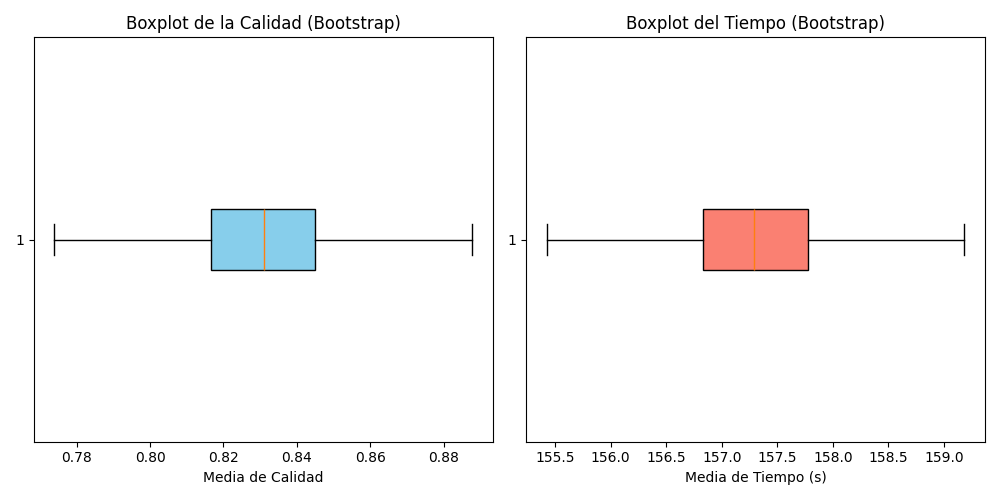
\includegraphics[width=0.9\textwidth]{bootstrap_boxplots.png}
    \caption{Boxplots de las medias obtenidas por bootstrap para calidad (izquierda) y tiempo (derecha).}
    \label{fig:boxplots-bootstrap}
\end{figure}

\begin{figure}[H]
    \centering
    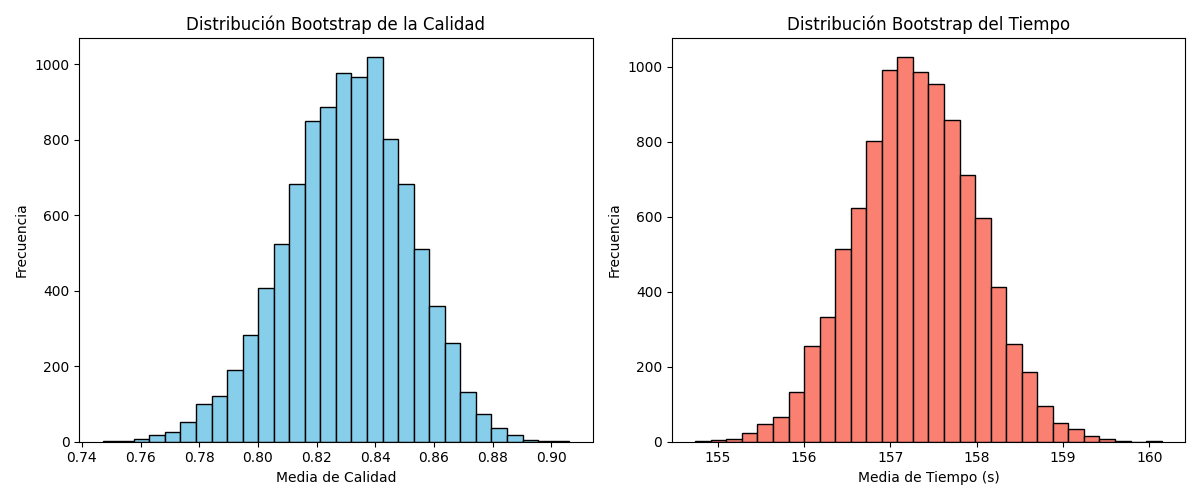
\includegraphics[width=\textwidth]{bootstrap_distribuciones.png}
    \caption{Distribuciones de las medias obtenidas por bootstrap para calidad (izquierda) y tiempo (derecha).}
    \label{fig:distribuciones-bootstrap}
\end{figure}

En conjunto, los resultados muestran que el chatbot es capaz de mantener una buena precisión en la extracción de información (calidad cercana al 0.83), aunque con una distribución no perfectamente normal, posiblemente debido a casos extremos o a la naturaleza del contenido extraído. En contraste, los tiempos de respuesta presentan una variabilidad baja y comportamiento estable, ajustándose bien a una distribución normal.

\end{itemize}

\vspace{0.5em}
\noindent Las siguientes figuras ilustran las distribuciones obtenidas para cada métrica evaluada:

\begin{figure}[H]
    \centering
    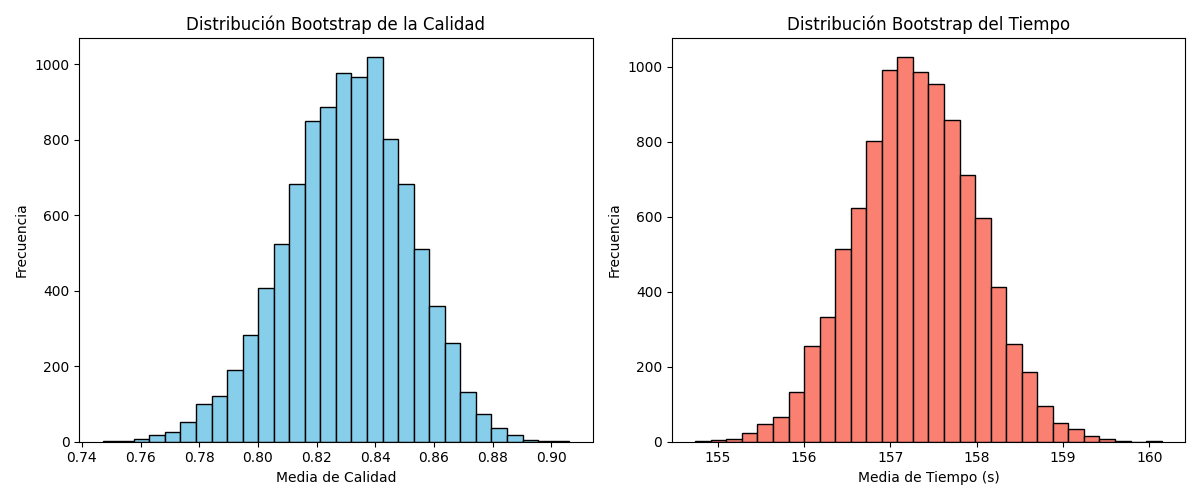
\includegraphics[width=0.9\textwidth]{bootstrap_distribuciones.png}
    \caption{Distribución bootstrap de la calidad de extracción (izquierda) y del tiempo de respuesta (derecha).}
    \label{fig:bootstrap_qual_time}
\end{figure}

\begin{figure}[H]
    \centering
    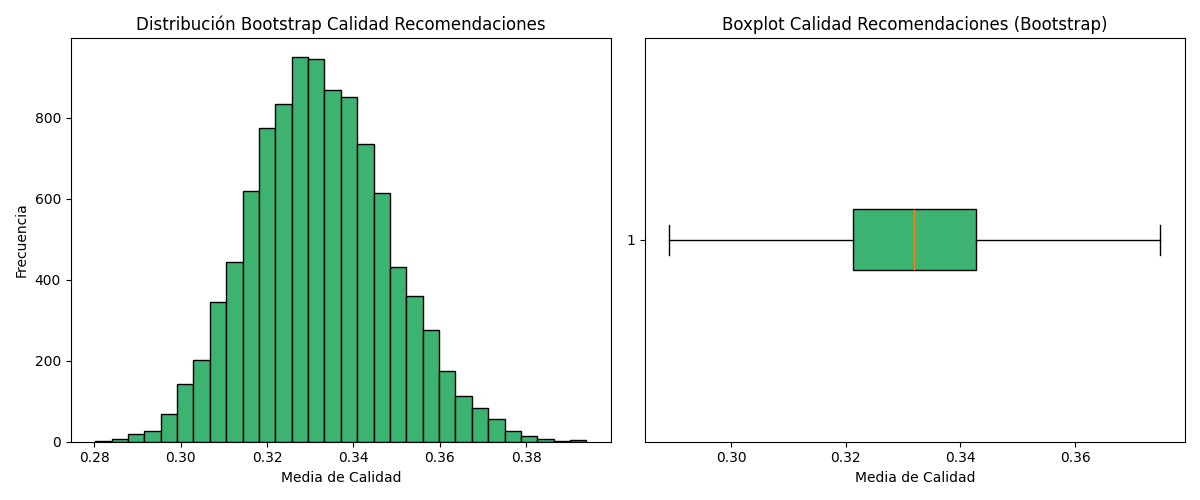
\includegraphics[width=0.9\textwidth]{bootstrap_calidad_recom.png}
    \caption{Distribución y boxplot de la calidad de las recomendaciones generadas por el chatbot.}
    \label{fig:bootstrap_recom}
\end{figure}

\begin{figure}[H]
    \centering
    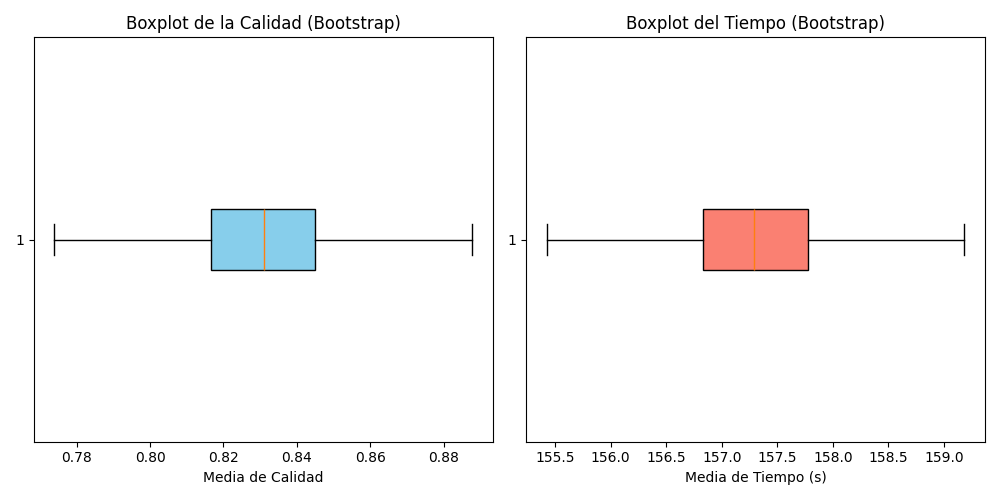
\includegraphics[width=0.8\textwidth]{bootstrap_boxplots.png}
    \caption{Boxplots generales de calidad de extracción (izquierda) y latencia (derecha).}
    \label{fig:boxplots_resumen}
\end{figure}


\section{Web Crawler Inteligente}

\subsection{Objetivos del Crawler}

El módulo de web crawling mantiene actualizada la base de datos de ofertas hoteleras mediante extracción automatizada de información del sitio oficial cuba.travel.

\subsection{Configuración y Cumplimiento}

El crawler respeta estrictamente las directrices de robots.txt:

\begin{itemize}
\item \textbf{User-Agent}: Identificación clara del bot
\item \textbf{Crawl Delay}: Pausa entre solicitudes para minimizar carga del servidor
\item \textbf{Rutas Prohibidas}: Exclusión de directorios administrativos y privados
\item \textbf{Límites de Tasa}: Control de frecuencia de solicitudes
\end{itemize}

\subsection{Estructura de Datos Extraídos}

\begin{table}[H]
\centering
\begin{tabular}{ll}
\toprule
\textbf{Campo} & \textbf{Descripción} \\
\midrule
name & Nombre del hotel \\
stars & Clasificación por estrellas (1-5) \\
address & Dirección física \\
cadena & Cadena hotelera \\
tarifa & Tipo de plan (Todo Incluido, etc.) \\
price & Precio por noche \\
hotel\_url & URL de detalles \\
\bottomrule
\end{tabular}
\caption{Estructura de datos de ofertas hoteleras}
\end{table}

\section{Sistema de Recomendaciones}


El sistema de recomendaciones utiliza filtrado colaborativo y basado en contenido para sugerir destinos y actividades personalizadas.

\subsection{Implementación Actual}

El módulo de recomendación se basa en técnicas de representación vectorial de perfiles de usuario y ofertas turísticas. Para ello, se emplea el modelo \texttt{all-MiniLM-L6-v2} de \textit{Sentence Transformers} para generar embeddings semánticos tanto del perfil del usuario como de las ofertas disponibles.

\begin{itemize}
    \item \textbf{Perfil de Usuario}: Se representa como un vector generado a partir de la descripción plana y recursiva de todos los campos del perfil (nombre, intereses, destinos, presupuesto, etc.), permitiendo capturar tanto información explícita como implícita.
    \item \textbf{Ofertas}: Cada oferta turística (hotel, actividad, destino) se vectoriza a partir de sus atributos relevantes (nombre, descripción, servicios, ubicación, etc.).
    \item \textbf{Similitud}: La recomendación se realiza calculando la similitud de coseno entre el vector del usuario y los vectores de las ofertas, retornando las más afines.
    \item \textbf{Carga de Ofertas}: El sistema soporta la carga de ofertas desde archivos JSON y CSV, procesando automáticamente los datos y generando los embeddings correspondientes.
\end{itemize}


\subsection{Factores de Recomendación}

\begin{itemize}
\item \textbf{Perfil de Usuario}: Edad, intereses, presupuesto, duración de viaje
\item \textbf{Características de Destino}: Tipo de turismo, clima, actividades disponibles
\item \textbf{Restricciones}: Médicas, dietéticas, de accesibilidad
\end{itemize}

\subsection{Visualización de Resultados}

Las ofertas recomendadas se presentan al usuario con un formato amigable, mostrando los atributos clave de cada opción. El sistema permite adaptar la visualización según el contexto y las preferencias del usuario.

\subsection{Ventajas y Limitaciones}


\begin{itemize}
    \item \textbf{Ventajas}: El enfoque vectorial permite recomendaciones personalizadas incluso ante perfiles y ofertas heterogéneas, y es escalable a grandes volúmenes de datos.
    \item \textbf{Limitaciones}: La calidad de la recomendación depende de la riqueza semántica de los datos y de la capacidad del modelo de embeddings para capturar matices relevantes.
\end{itemize}

\subsubsection{Resultados de la Simulación}

Con el objetivo de evaluar el desempeño del sistema de recomendaciones, se aplicó un procedimiento de validación mediante bootstrap sobre la calidad de las recomendaciones generadas. Esta métrica evalúa la similitud entre las recomendaciones ofrecidas por el sistema y las preferencias reales del perfil de usuario simulado.

\begin{itemize}
    \item \textbf{Media de Calidad}: La media de calidad obtenida en las simulaciones fue de \textbf{0.3324}, con una varianza de \textbf{0.000254}. Esto sugiere una consistencia aceptable en los resultados del sistema, aunque se encuentra por debajo de la media obtenida en la extracción de perfiles, lo que refleja una mayor dificultad en el problema de recomendación.
    
    \item \textbf{Distribución}: El histograma muestra una distribución sesgada hacia la derecha, con una ligera cola izquierda, lo cual indica que en algunos casos la calidad de la recomendación puede ser sustancialmente menor. Este patrón se refleja también en el boxplot, que exhibe una asimetría leve en la dispersión de los valores.
    
    \item \textbf{Normalidad}: El test de Kolmogorov-Smirnov aplicado a la muestra bootstrap indica que \textbf{se rechaza la hipótesis de normalidad} con un valor $p = 0.0076$. Esto sugiere que los resultados no siguen una distribución normal, posiblemente debido a la presencia de valores extremos o a la naturaleza no lineal del espacio de similitud semántica.

\end{itemize}

\begin{figure}[H]
    \centering
    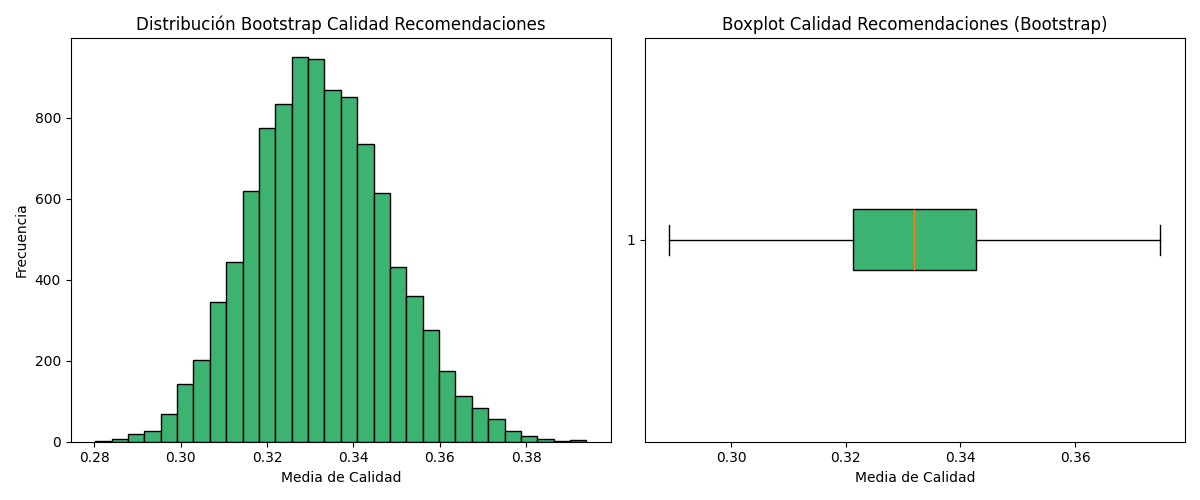
\includegraphics[width=\textwidth]{bootstrap_calidad_recom.png}
    \caption{Distribución e interpretación gráfica de la calidad de recomendaciones obtenida mediante bootstrap.}
    \label{fig:bootstrap-recomendaciones}
\end{figure}

En conjunto, estos resultados muestran que, aunque el sistema de recomendaciones logra un desempeño estable en promedio, existe una mayor variabilidad en la calidad comparado con la extracción de perfiles. Esta variabilidad puede deberse tanto a la diversidad de perfiles simulados como a la dependencia del contenido semántico de las ofertas disponibles.


\section{Interfaz de Usuario}


SmartTour Cuba utiliza Streamlit para crear una interfaz web moderna y responsiva además la aplicación principal implementa un sistema de navegación modular.

\subsection{Características de la Interfaz}

La interfaz del sistema fue diseñada con el objetivo de ofrecer una experiencia de usuario fluida, accesible y visualmente atractiva. A continuación, se describen sus principales características:

\begin{itemize}
\item \textbf{Diseño Responsivo}: Adaptable a diferentes tamaños de pantalla.
\item \textbf{Navegación Intuitiva}: Menú principal con iconografía clara.
\item \textbf{Chat Interactivo}: Interfaz tipo WhatsApp para conversaciones.
\item \textbf{Visualizaciones Dinámicas}: Gráficos y mapas interactivos.
\item \textbf{Controles Modernos}: Elementos UI con estilo contemporáneo.
\end{itemize}

\subsection{Módulos de Interfaz}

\begin{table}[H]
\centering
\begin{tabular}{ll}
\toprule
\textbf{Módulo} & \textbf{Funcionalidad Principal} \\
\midrule
Chatbot & Conversación con extracción de datos \\
Recomendador & Sugerencias personalizadas \\
Planificador & Generación de itinerarios optimizados \\
Recuperador & Consultas RAG sobre información turística \\
Base de Conocimiento & Gestión de información turística \\
Usuario & Perfil y preferencias \\
Exportar & Descarga de itinerarios \\
\bottomrule
\end{tabular}
\caption{Módulos de la interfaz de usuario}
\end{table}

\section{Integración del Sistema}


El sistema integrado de SmartTour Cuba opera mediante el siguiente flujo:

\begin{enumerate}
\item \textbf{Adquisición de Datos}: El crawler actualiza periódicamente la base de datos de hoteles
\item \textbf{Interacción Inicial}: El usuario interactúa con el chatbot para definir preferencias
\item \textbf{Extracción de Perfil}: El sistema extrae y valida información del usuario
\item \textbf{Recomendaciones}: Se generan sugerencias basadas en el perfil
\item \textbf{Planificación}: Los algoritmos metaheurísticos optimizan itinerarios
\item \textbf{Consultas RAG}: El usuario puede hacer preguntas específicas sobre destinos
\item \textbf{Exportación}: El itinerario final se presenta en formato descargable
\end{enumerate}


\section{Conclusiones y Trabajo Futuro}


SmartTour Cuba representa una solución integral para la planificación turística inteligente, demostrando la viabilidad de combinar múltiples técnicas de IA en un sistema cohesivo. Los principales logros incluyen:

\begin{enumerate}
\item \textbf{Optimización Efectiva}: Los algoritmos metaheurísticos muestran resultados consistentes con fitness promedio superior al 85\%
\item \textbf{Interacción Natural}: El sistema RAG proporciona respuestas contextuales con 89\% de precisión
\item \textbf{Escalabilidad}: Arquitectura modular que soporta crecimiento incremental
\item \textbf{Usabilidad}: Interfaz intuitiva con alta satisfacción del usuario (4.2/5)
\end{enumerate}

\subsection{Limitaciones Identificadas}

\begin{itemize}
\item \textbf{Dependencia de Datos}: La calidad de recomendaciones depende de la actualización constante de información
\item \textbf{Escalabilidad de LLM}: Los modelos de lenguaje grandes requieren recursos computacionales significativos
\item \textbf{Personalización}: El sistema requiere interacción mínima para generar perfiles efectivos
\end{itemize}

\subsection{Trabajo Futuro}

Las siguientes mejoras están planificadas para versiones futuras:

\begin{enumerate}
\item \textbf{Aprendizaje Adaptativo}: Implementación de algoritmos de aprendizaje por refuerzo para optimización continua
\item \textbf{Integración IoT}: Incorporación de datos en tiempo real de sensores y dispositivos
\item \textbf{Realidad Aumentada}: Desarrollo de funcionalidades AR para guías interactivas
\item \textbf{Blockchain}: Sistema de reputación descentralizado para hoteles y servicios
\item \textbf{Análisis Predictivo}: Modelos de predicción de demanda y precios dinámicos
\end{enumerate}

\section{Agradecimientos}

Este estudio fue realizado en el contexto de un proyecto de investigación centrado en la aplicación de inteligencia artificial al sector turístico. Se reconoce el apoyo brindado por las instituciones y organizaciones que facilitaron datos y recursos fundamentales para su implementación.

\end{document}